%定义文档类为beamer,选项设置为draft可以加快编译速度
%\documentclass[draft]{beamer} 
\documentclass[UTF8, compress]{ctexbeamer}



%---------------导入外部宏包----------------%
%beamer文档类会自动调用`amsmath`宏包,此处不再重复调用



%导入绘图包
\usepackage{tikz}
\usetikzlibrary{fadings}

%插图
\usepackage{graphicx, float}

%代码高亮
\usepackage{xcolor, listings}

%插入手势符号与数学符号
\usepackage{amssymb, pifont}


%设置代码环境基本参数
\lstset
{
	breaklines=true,
	tabsize=3,
	showstringspaces=false
}


\lstdefinestyle{Common}
{
	extendedchars=\true,
	language={R},
	frame=shadowbox,
	%===========================================================
	framesep=3pt,%expand outward.
	framerule=0.4pt,%expand outward.
	xleftmargin=3.4pt,%make the frame fits in the text area. 
	xrightmargin=3.4pt,%make the frame fits in the text area.
	%=========================================================== 
	rulecolor=\color{blue!90}
}

\lstdefinestyle{A}
{
	style=Common,
	%basicstyle=\scriptsize\color{black}\ttfamily,
	basicstyle=\small\color{black}\ttfamily,
	keywordstyle=\color{blue},
	identifierstyle=\color{teal},
	stringstyle=\color{violet},
	commentstyle=\color{darkgray}
}

%-------------------设置Beamer主题----------------------%
% 主题设置:华沙
\usetheme{Warsaw}


\usetheme{Darmstadt} 
%\useoutertheme[subsection=false,footline=authortitle]{miniframes}
%\setbeamertemplate{navigation symbols}{} 





%外部主题设置:设置显示顶部导航区:信息行
\useoutertheme{infolines}



%-----------设置字体--------------%
%设置默认字体为衬线字体,即:中文宋体,英文衬线字体
\usefonttheme{serif}
%设置特殊环境中的字体随环境显示
\usefonttheme{professionalfonts}







%设置标题页的内容显示
\title{{\heiti 多维标度法}{\sffamily MDS}{\heiti 及}{\sffamily R}{\heiti 使用}}
\author{Apocalypse}
\date{\heiti 2020年10月9日}
\institute[{\sffamily CUGB}]{\heiti 中国地质大学(北京) \quad 数理学院}


\begin{document}

	
	%设置标题页
	\begin{frame}
		\titlepage
	\end{frame}
	
	%设置目录页
	\begin{frame}
		\frametitle{\heiti 内容提要}
		\tableofcontents 
		%后加[pausesections]选项可以逐帧显示目录
	\end{frame}
	
%正文部分		
\section{{\heiti 问题引入与背景简介}}
	% 其他目录显示为灰色,只突出显示当前节(section),下同
	\frame{\tableofcontents[currentsection]}
	\begin{frame}
	\frametitle{\heiti 问题引入}
		\begin{exampleblock}<1->{\heiti 问题}<2->
			有$n$个由多个指标反映的客体,但反映这些客体的指标个数未知,甚至指标本身就是模糊的,我们仅知道这$n$个客体间的某种距离(不一定是通常的欧氏距离)或某种相似性。\\
			\vspace{.25cm}
			\onslide<3->
			我们希望仅由这种距离或相似性给出的信息出发,在较低维度的欧氏空间中把这$n$个客体(作为几何点)的图形绘制出来,从而尽可能及时地反映这些客体之间真实的结构关系。
		\end{exampleblock}
		
		\onslide<4->
			\vspace{0.5cm}
			多维标度 (Multi-Dimensional Scaling,\ MDS) 分析是以空间分布的形式表现对象之间相似性或亲疏关系的一种多元数据分析方法。其结果主要是\textbf{偏好图}(又称多维标度图)等。\\
			
		\onslide<5->
			\vspace{.5cm}
			MDS 分析多见于市场营销领域,近年来在经济管理领域的应用也日趋增多。
	\end{frame}



\section{{\sffamily MDS} {\heiti 的概念和方法}}
	\frame{\tableofcontents[currentsection]}
	
	\begin{frame}
%		添加帧标题
	\frametitle{\heiti \textsf{MDS}的基本概念}
	
		\begin{block}<1->{\heiti 定义}<2->
			\textbf{多维标度法}是利用客体间的\textbf{相似性数据}去揭示它们之间\textbf{空间关系}的统计分析方法。
		\end{block}

		\onslide<3->
		
		根据所分析数据的类型,可将多维标度法分为度量化模型和非度量化模型:

		\begin{itemize}
			\item<4-> 度量化模型(Metric MDS) \\

			若模型所需要的相似性数据是用\alert{距离尺度}或\alert{比率尺度}测得的,则称此模型为\textbf{度量化模型}。
			
			\vspace{0.25cm}
			
			\item<5->非度量化模型(Nonmetric MDS) \\ 

			若模型需要\alert{顺序量表水平}的相似数据,称此模型为\textbf{非度量化模型}。
		\end{itemize}
	
		\begin{block}<5->{\heiti 基本思想}<6->
			将高维坐标中的点投影到低维空间中,保持点彼此之间的相似性尽可能不变。
		\end{block}
	
	\end{frame}


	\begin{frame}
		\begin{exampleblock}<1->{\heiti 例1}<2->
			下表是美国10个城市间的公路距离(并非直线距离),我们希望在地图上重新标出这$10$个城市,使得它们之间的距离接近表中的距离。
			\begin{figure}
				\centering
				\includegraphics[width=1\linewidth]{figures/tabular1}
			\end{figure}
		\end{exampleblock}
	
		\onslide<3-> 
		如果用$D=(d_{ij})$表示上表的矩阵,虽然名义上是距离阵,但不一定是$n$个点的距离,所以下面我们扩展距离矩阵的定义。
	
	\end{frame}




	\begin{frame}
		%	添加帧标题
		\frametitle{\heiti \textsf{MDS}的基本方法}
		
%		添加定义
		\begin{block}<1->{\heiti 定义}<2->
			一个$n\times n$矩阵$D=(d_{ij})$,若满足 $D^T=D$, $\,d_{ii}=0$, $\,d_{ij}\geqslant0$, $\,(i,\,j=1,\,2,\,\cdots,\,n;\,i\neq j)$,则称 $\!D\!$ 为\textbf{距离阵}。
		\end{block}
		
		
		\onslide<3-> 
		
			对于距离阵$D=(d_{ij})$,多维标度法的目的是寻找$p$和$\mathbb{R}^p$中的$n$个点$x_1,\,x_2,\,\cdots,\,x_n$,用$\widehat{d}_{ij}$表示$x_i$与$x_j$的欧氏距离,$\widehat{D}=(\widehat{d}_{ij})$,使得$\widehat{D}$与$D$在某种意义下相近。
			
			\vspace{0.5cm}
			
		
		\onslide<4->
			
			在实际运用中,常取$p=1,\,2,\,3$.
			将寻找到的$n$个点$x_1,\,x_2,\,\cdots,\,x_n$写成矩阵形式如下:
		
		\onslide<5->
		
		\begin{equation}
		X=(x_1,\,x_2,\,\cdots,\,x_n)^T
		\end{equation}
		
		\onslide<6->
		
		则称$X$为$D$的一个解(或称\textbf{多维标度解})。
	
	\end{frame}




\section{{\sffamily MDS} {\heiti 的古典解}}
	\frame{\tableofcontents[currentsection]}
	
	\begin{frame}
	\frametitle{\heiti 欧式型距离阵及其判定定理}
		
		\begin{block}<1->{\heiti 定义:欧式型距离阵}<2->
			
			一个距离阵$D=(d_{ij})$称为\textbf{欧式型}的,若存在某个正整数$p$及$p$维空间$\mathbb{R}^p$中的$n$个点 $x_1,\,\cdots,\,x_n$,\ 使得
			
			
			\begin{align}
			\uncover<3-> {d^2_{ij} &= (x_i-x_j)'(x_i-x_j), \\}
			\uncover<4-> {A &= (a_{ij}),\ \ \,\ a_{ij}=-\frac12d_{ij}^2, \\}
			\uncover<5-> {B &= H'AH,\ H=I_n-\frac1n1_n1'_n. \label{eq4}\\}
			\notag
			\end{align}
		
		\end{block}
		
		
		\begin{block}<5->{\heiti 定理: 欧式型距离阵判定定理}<6->
			一个$n\times n$的距离阵$D$是欧式型的充要条件是:$B\geqslant0$.
		\end{block}
	
	\end{frame}
	
	\begin{frame}
	\frametitle{\heiti 谱分解定理}
	
	
		\begin{block}<1->{\heiti 定义: 矩阵的谱}<2->
			矩阵$A$的所有特征值的全体$\lambda_1,\,\cdots,\,\lambda_n$称为矩阵$A$的谱,记为$\lambda(A)$。
		\end{block}

		\vspace{.5cm}

		\begin{block}<2->{\heiti 定理: 谱分解定理}<3->
			设$\!A\geqslant0\!$为对称矩阵,$\!\lambda_i,\,\lambda_j\!$是$A$的两个相异特征根,相应的特征向量$\ell_i$和$\ell_j$相互正交,则$\!A\!$可表示为$\!A=T\Lambda T'=\sum\limits_{i=1}^p\lambda_i\ell_i\ell_i'$,称为矩阵$\!A\!$的\textbf{谱分解}。
			\pause
			即存在一个正交阵$T$,使$T'AT=\mathrm{diag}(\lambda_1,\,\lambda_2,\,\cdots\,\lambda_p)=\Lambda$,其中$T$的列向量为相应的特征向量。
		\end{block}
	\end{frame}

	\begin{frame}
		\textbf{\heiti 证明:}	
		\pause
			(必要性) 设距离阵$D$是欧式型的,则由欧式型距离阵的定义可知,存在$x_1,\,\cdots,\,x_n\in\mathbb{R}^p$,使得
			\begin{equation}
			\label{eq5}
			d_{ij}^2=-2a_{ij}=(x_i-x_j)'(x_i-x_j),
			\end{equation}
		\pause
			由\eqref{eq4}可得:
			\begin{equation}
			\label{eq6}
			B=H'AH=A-\dfrac1nAJ-\dfrac1nJA+\dfrac1{n^2}JAJ,
			\end{equation}
			上式中,$J=1_n1_n'$。
		\pause		
			并注意到
			\begin{equation}
			\dfrac1nAJ=\begin{bmatrix}
			\bar{a}_{1.}\\
			\bar{a}_{2.}\\
			\vdots\\
			\bar{a}_{n.}
			\end{bmatrix}
			1_n',\ 
			\dfrac1nJA=1_n(\bar{a}_{.1},\,\bar{a}_{.2},\,\cdots,\,\bar{a}_{.n}),\ 
			\dfrac1{n^2}JAJ=\bar{a}_{..}1_n1_n',
			\end{equation}			
		\pause			
			其中,
			\begin{equation}
			\bar{a}_{i.}=\dfrac1n\sum\limits_{j=1}^na_{ij},\ 
			\bar{a}_{.j}=\dfrac1n\sum\limits_{i=1}^na_{ij},\ 
			\bar{a}_{..}=\dfrac1{n^2}\sum\limits_{i=1}^n\sum\limits_{j=1}^na_{ij}.
			\end{equation}
	
	\end{frame}

	\begin{frame}
		\pause
			将上述各式代入\eqref{eq6},得到
			\begin{equation}
			\label{eq8}
			b_{ij}=a_{ij}-\bar{a}_{i.}-\bar{a}_{.j}+\bar{a}_{..},
			\end{equation}
		\pause
			再由\eqref{eq5}式可分别求得$a_{ij},\,\bar{a}_{i.},\,\bar{a}_{.j},\,\bar{a}_{..}$,将其代入式\eqref{eq8},得到
			\begin{equation}
			b_{ij}=(x_i-\bar{x})'(x_i-\bar{x})\geqslant0,
			\end{equation}
			其中$\bar{x}=\dfrac1n\sum\limits_{i=1}^nx_i$,
		\pause
			将上式写成矩阵形式,即得到
			\begin{equation}
			B=(HX)(HX)'\geqslant 0
			\end{equation}
			必要性得证,下证充分性。\\
		\pause
		
			\vspace{.5cm}
			(充分性) 记$p=\mathrm{rank}(B),\,\lambda_1,\,\lambda_2,\,\cdots,\,\lambda_p$为$B$的正特征根,$x_{(1)},\,\cdots,\,x_{(p)}$为对应的特征向量。
	\end{frame}


	\begin{frame}
		
		
		\pause
			由已知条件,$B\geqslant0$,根据\textbf{谱分解定理}得到
			\begin{equation}
			B=H'AH=\varGamma\Lambda\varGamma'
			\end{equation}
			其中$\Lambda=\mathrm{diag}(\lambda_1,\,\lambda_2,\,\cdots,\,\lambda_p),\,\lambda_1\geqslant\cdots\geqslant\lambda_p$为$B$的$p$个正特征根$\varGamma=X\Lambda^{-\frac12},\,\varGamma$的$p$个列为对应的$p$个标准正交化的特征向量。
		\pause
			取$X=\varGamma\Lambda^{\frac12}$,为一$n\times p$阶矩阵。将$X$写成$X=(x_1,\,x_2,\,\cdots,\,x_n)'=(x_{(1)},\,x_{(2)},\,\cdots,\,x_{(p)})$,于是有
			\begin{equation}
			X'X=(\varGamma\Lambda^{\frac12})'(\varGamma\Lambda^{\frac12})=\Lambda,\ B=XX',
			\end{equation}
			即$b_{ij}=x_i'x_j$。
		\pause
			由此得到$x_i$与$x_j$两点的距离平方
			\begin{align}
			(x_i-x_j)'(x_i-x_j) 
			&= x_i'x_i-2x_i'x_j+x_j'x_j=b_{ii}-2b_{ij}+b_{jj}\\
			&= a_{ii}-2a_{ij}+a_{jj}= -2a_{ij}=d_{ij}^2
			\end{align}
		\pause
			根据上述推导可知:存在正整数$p$和一个$n\times p$阶矩阵$X=(x_1,\,x_2,\,\cdots,\,x_n)=\varGamma\Lambda^{\frac12}$,使得$X$是$D$的构造点,所以$D$为欧式型。\qed
	\end{frame}



	\begin{frame}
	\frametitle{\heiti MDS 古典解的计算步骤$\bigstar$}
		\onslide<1->
		\begin{enumerate}
			\item<2-| alert@2> 由距离阵$D=(d_{ij})$ 构造矩阵$A=(a_{ij})=-\dfrac12d_{ij}^2$;
			
			\item<3-| alert@3> 令矩阵$B=(b_{ij})$,\ 其中$b_{ij}=a_{ij}-\overline{a}_{i.}-\overline{a}_{.j}+\overline{a}_{..}$;
			
			\item<4-| alert@4>
			求矩阵$B$的特征根$\lambda_1\geqslant\lambda_2\geqslant\cdots\geqslant\lambda_n$,\ 若无负特征根,表明$B\geqslant 0$,\ 从而距离阵$D$是欧式型的;\ 若有负特征根,距离阵$D$一定不是欧式型的。
			
			\onslide<5->
			此时令
			\begin{equation}
			a_{1,\,k}=
			\dfrac{\sum\limits_{i=1}^k\lambda_i}{\sum\limits_{i=1}^n|\lambda_i|},\quad
			a_{2,\,k}=
			\dfrac{\sum\limits_{i=1}^k\lambda_i^2}{\sum\limits_{i=1}^n\lambda_i^2},
			\end{equation}
			
			\onslide<6->
			上面两个量相当于主成分分析(PCA)中的\textbf{累积贡献率};
			
			
			\item<7-| alert@7> 令$\hat{X}
			=\big(\hat{x}_{(1)},\,\cdots,\,\hat{x}_{(k)}\big)$,\ 则$\hat{X}$的行向量$x_1,\,\cdots,\,x_n$
			即为欲求的古典解。
		\end{enumerate}
	\end{frame}
	
	
	\begin{frame}
		
		\begin{exampleblock}<1->{\heiti 例2}<2->
			设有距离阵$D$如下,计算MDS的古典解。
			\begin{equation}
			D=
			\begin{bmatrix}
			\begin{smallmatrix}
				0 & 1 & \sqrt3 & 2 & \sqrt3 & 1 & 1 \\
				& 0 & 1 & \sqrt3 & 2 & \sqrt3 & 1 \\
				&   & 0 & 1 & \sqrt3 & 2 & 1 \\
				&   &   & 0 & 1 & \sqrt3 & 1 \\
				&   &   &   & 0 & 1 & 1 \\
				&   &   &   &   & 0 & 1 \\
				&   &   &   &   &   & 0 \\
			\end{smallmatrix}
			\end{bmatrix}
			\end{equation}
			
		\end{exampleblock}
	
		\onslide<3->
		
		根据上述计算步骤,有$a_{ij}=-\frac12d_{ij}^2$,由此得到
		
		\onslide<4->
		
		\begin{equation}
		A=
		\begin{bmatrix}
		\begin{smallmatrix}
			0 & -\frac12 & -\frac32 & -2 & -\frac32 & -\frac12 & -\frac12 \\[3pt]
			& 0 & -\frac12 & -\frac32 & -2 & -\frac32 & -\frac12 \\[3pt]
			&   & 0 & -\frac12 & -\frac32 & -2 & -\frac12 \\[3pt]
			&   &   & 0 & -\frac12 & -\frac32 & -\frac12 \\[3pt]
			&   &   &   & 0 & -\frac12 & -\frac12 \\[3pt]
			&   &   &   &   & 0 & -\frac12 \\[3pt]
			&   &   &   &   &   & 0 \\
		\end{smallmatrix}
		\end{bmatrix}
		\end{equation}
	
	\end{frame}
	
	\begin{frame}
		再由$b_{ij}=a_{ij}-\overline{a}_{i.}-\overline{a}_{.j}+\overline{a}_{..}$,得到
		\pause
		\begin{equation}
		2B=
		\begin{bmatrix}
		\begin{smallmatrix}
		2 & 1 & -1 & -2 & -1 & 1 & 0 \\[3pt]
		1 & 2 & 1 & -1 & -2 & -1 & 0 \\[3pt]
	   -1 & 1 & 2 & 1 & -1 & -2 & 0 \\[3pt]
	   -2 & -1 & 1 & 2 & 1 & -1 & 0 \\[3pt]
	   -1 & -2 & -1 & 1 & 2 & 1 & 0 \\[3pt]
		1 & -1 & -2 & -1 & 1 & 2 & 0 \\[3pt]
		0 & 0 & 0 & 0 & 0 & 0 & 0 \\
		\end{smallmatrix}
		\end{bmatrix}
		\end{equation}
		\pause
		
		计算矩阵$B$的特征根,并按从大到小排序:$\lambda_1=\lambda_2=3$,\ $\lambda_3=\cdots=\lambda_7=0$。$B$无负特征根,说明$B\geqslant0$,所以$D$是欧式型的。
		
		\pause
		
		计算特征向量,得$x_{(1)}=(0,\,-a,\,-a,\,0,\,a,\,a,\,0)^T$,\ $a=\frac{1}2$, \ $x_{(2)}=(-2b,\,-b,\,b,\,2b,\,b,\,-b,\,0)^T$,\ $b=\frac{\sqrt3}2$。
		\pause
		所以可得七个点的坐标分别为:$(0,\,-\sqrt3),\ (-\frac12,\,-\frac{\sqrt3}2),\ (-\frac12,\,\frac{\sqrt3}2),\ (0,\,\sqrt3),\ (\frac12,\,\frac{\sqrt3}2),\ (\frac12,\,-\frac{\sqrt3}2),\ (0,\,0)$, \\
		\vspace{.2cm}
		此即$D$的古典解。
		
	\end{frame}
	
	
	\begin{frame}[fragile]
	\frametitle{{\sffamily MDS}{\heiti 古典解的}{\sffamily R}{\heiti 实现}}
		\pause
		
\begin{lstlisting}[style=A]
cmdscale(d, k = 2, eig = FALSE, add = FALSE, x.ret = FALSE, list. = eig || add || x.ret)
\end{lstlisting}

		\pause
		
		\vspace{.3cm}
		
		$d$表示进行多维标度分析的距离矩阵,$k$表示维度,默认取$2$维.
		\pause
		下面应用R中自带的函数\textbf{cmdscale()},对上述例题进行MDS古典解的计算。
		
		\pause
		
\begin{lstlisting}[style=A]
D <- matrix(c(0,1,sqrt(3),2,sqrt(3),1,1,
              1,0,1,sqrt(3),2,sqrt(3),1,
              sqrt(3),1,0,1,sqrt(3),2,1,
              2,sqrt(3),1,0,1,sqrt(3),1,
              sqrt(3),2,sqrt(3),1,0,1,1,
              1,sqrt(3),2,sqrt(3),1,0,1,
              1,1,1,1,1,1,0), nrow = 7)
result <- round(cmdscale(D), 3); result
plot(result)
\end{lstlisting}

	\end{frame}



	\begin{frame}[fragile]

		运行结果:
		\pause
\begin{lstlisting}
 [,1] [,2]
[1,]  0.000  1.0
[2,] -0.866  0.5
[3,] -0.866 -0.5
[4,]  0.000 -1.0
[5,]  0.866 -0.5
[6,]  0.866  0.5
[7,]  0.000  0.0
\end{lstlisting}
		\pause
		\vspace{-.25cm}
		\begin{figure}[H]
			\centering
			\includegraphics[width=4.5cm]{figures/1}
			\qquad
			\includegraphics[width=4.5cm]{figures/2}
		\end{figure}
		
	\end{frame}

	\begin{frame}[fragile]
		\pause
		
		另一种方法也可以得出同样的结论,根据前面定理证明的方法。下面具体讲解。
		
		\pause
		
\begin{lstlisting}[style=A]
calc_mds <- function(D) {
    dim <- nrow(D)
    A <- -1/2*D^2
    onen <- matrix(rep(1, dim), nrow=dim)
    H <- diag(dim) - 1/dim * onen %*% t(onen)
    B <- t(H) %*% A %*% H
    val <- eigen(B, symmetric=F)$values
    vec <- eigen(B, symmetric=F)$vectors
    MDS <- vec[,1:2] %*% diag(sqrt(val[1:2])); 
    data.frame(points = round(MDS, 3))
}
MDS <- calc_mds(D)
plot(MDS)
\end{lstlisting}
		
	\end{frame}
	
	
	
	\begin{frame}[fragile]
		\begin{exampleblock}<1->{\heiti 例 3 }<2->
			考虑例 1 中美国10个城市的距离阵,计算其MDS古典解。
		\end{exampleblock}
		\vspace{-.2cm}
		\onslide<3->
		
\begin{lstlisting}[style=A]
X <- openxlsx::read.xlsx("mvstats4.xlsx", sheet="d12.1", rowNames = T)
B <- calc_mds(as.matrix(X))
# 自编函数计算累积贡献率
calc_acr <- function(lambda, k) {
    a1k <- sum(lambda[1:k]) / sum(abs(lambda))
    a2k <- sum(lambda[1:k]^2) / sum(lambda^2)
    list(a1k=round(a1k, 3), a2k=round(a2k, 3))
}
calc_acr(eigen(B)$values, 2)
MDS <- round(cmdscale(X), 2)# 计算古典解
# 图形绘制
plot(-MDS[, 1], -MDS[, 2], type = "n", asp = 1)
text(-MDS[, 1], -MDS[, 2], labels = rownames(X), cex=1.5)
\end{lstlisting}
		
	\end{frame}
	
	
	\begin{frame}
		\pause
		上述代码运行后可绘制如下图形,对比发现 MDS 准确度较高。
		\vspace{.2cm}
		\pause 
		\begin{figure}
			\centering
			\includegraphics[width=7.5cm]{figures/3}
			\includegraphics[width=7.5cm]{figures/4}
		\end{figure}
		
	\end{frame}
	
	
	
	\begin{frame}
	\frametitle{\heiti 古典解的优良性}
	
		\onslide<1->
		由{欧式型距离阵的判定定理}可知,距离阵$D$在$k$维实数空间中拟合构造点的古典解就是$X$的$k$维主坐标。
		
		\vspace{0.5cm}	
	
		\begin{block}<1->{\heiti 定理 2}<2->
			$X$ 的$k$维主坐标是将$X$中心化后$n$个样本的前$k$个主成分的值。
		\end{block}
	\end{frame}
	
\section{{\sffamily MDS} {\heiti 非度量方法}}

	\frame{\tableofcontents[currentsection]}
	
	\begin{frame}
		\frametitle{\heiti 非度量方法}
		
		\begin{enumerate}
			\item<1-> 度量化模型
			
			古典解(基于主成分分析的思想):
			\begin{equation*}
			d_{ij}=\widehat{d}_{ij}+\varepsilon_{ij}
			\end{equation*}
		\pause
			式中,$\widehat{d}_{ij}$是拟合$d_{ij}$的值,$\varepsilon_{ij}$为误差。
			\vspace{1cm}
			
			\item<3-> 非度量化模型
			
			非古典解:
			\begin{equation*}
			d_{ij}=f\big(\widehat{d}_{ij}+\varepsilon_{ij}\big)
			\end{equation*}
		\onslide<4->
			式中,$f$为一个未知的单调增加的函数。此时只能用$|d_{ij}|$的秩来构造$\widehat{d}_{ij}$.
		
		\end{enumerate}
	\end{frame}
	
	
	\begin{frame}
		\frametitle{{\sffamily Shepard-Kruskal} {\heiti 算法}}
		
		\begin{enumerate}
			\item<1-> 已知相似系数矩阵$D=(d_{ij})$,将其非对角元素由从小到大顺序排列起来:
			$d_{i_1j_1}\leqslant d_{i_2j_2}\leqslant \cdots \leqslant d_{i_mj_m}$,\  
			$m=\frac12n(n-1)$,\ $i_l<j_l$,\ 
			$l=1,\,2,\,\cdots,\,m$; 
			
			\item<2-> 设$\widehat{X}_{n\times k}$是$k$维拟合构造点,相应的距离阵$\widehat{D}=(\widehat{d}_{ij})$,\ 令
			
			\onslide<3->
			\begin{equation}
			S^2(\widehat{X})=\dfrac{\min\sum\limits_{i<j}(d_{ij}^*-\widehat{d}_{ij})^2}{\sum\limits_{i<j}d_{ij}^2}; 
			\end{equation}
			
			\item<4-> 若$k$固定,且能存在一个$\widehat{X}_0$,使得
			$S(\widehat{X}_0)=\min\limits_{\widehat{X}_{n\times k}}S(\widehat{X})\equiv S_k$,\ 则称$\widehat{X}_0$为$k$维最佳拟合构造点; 
			
			\item<5-| alert@5> 由于$S_k$(称为压力指数stress)是$k$的单调下降序列,取$k$使$S_k$适当小。
			
			\onslide<6-> \alert{例如$S_k<5\%$最好,$5\%\leqslant S_k \leqslant 10\%$次之,$S_k>10\%$较差。}
		\end{enumerate}

	\end{frame}

	\begin{frame}[fragile]
	\frametitle{{\sffamily MDS}{\heiti 非度量方法的}{\sffamily R}{\heiti 实现}}
	
	\pause 
	
\begin{lstlisting}[style=A]
# 需要导入MASS包
isoMDS(d, y = cmdscale(d, k), k = 2, maxit = 50, trace = TRUE, tol = 1e-3, p = 2)
Shepard(d, x, p = 2)
\end{lstlisting}

	\pause 
	\vspace{.3cm}
	
	$d$表示进行多维标度分析的距离矩阵,$k$表示维度,默认取$2$维.
	
	\vspace{.3cm}
	
	\pause
	
	\textbf{Shepard()}函数用于比较MDS结果的好坏。
	作图后,折线越趋近于一条平滑的斜线表明MDS降维的效果越好。
	

	\end{frame}

	
\section{{\sffamily MDS} {\heiti 的计算过程}}

	\frame{\tableofcontents[currentsection]}
	
	\begin{frame}
	\frametitle{\heiti 多维标度法的计算过程小结}
		
		\begin{tikzpicture}
		
		\visible<1->{
		
		\fill[cyan!20] (-3, 0) arc (90:-90:3); 
		\node [black, font=\LARGE] at (-1.75, -3) {\heiti \begin{tabular}{c}
			计 \\ 算 \\ 步 \\ 骤
			\end{tabular}};
		\draw[gray!30, line width=3pt] (-3, .25) arc (90:-90:3.25);
	}
		
		\visible<2->{
			
		\fill[color=cyan!30!white] (-.8, -.5) ellipse (.22 and .28) node [black] {1};
		\shadedraw[lightgray] (-.25, -.8) rectangle (2.85, -.2) 
		node[right, black] at (-.25, -.5) {\heiti \,确定研究的目的};
	}
		
		
		\visible<3->{
		
		\fill[color=cyan!30!white] (0, -1.5) ellipse (.22 and .28) node [black] {2};
		\shadedraw[lightgray] (.8, -1.8) rectangle (4, -1.2)
		node[right, black] at (.75, -1.5) {\heiti \,\,选择样品和变量};
	} 
		
		
		\visible<4->{
		
		\fill[color=cyan!30!white] (.25, -2.5) ellipse (.22 and .28) node [black] {3};
		\shadedraw[lightgray] (1, -2.8) rectangle (5.15, -2.2) 
		node[right, black] at (1, -2.5) {\heiti 计算样品间的距离矩阵};
	}
		
		
		\visible<5->{
		
		\fill[color=cyan!30!white] (.25, -3.5) ellipse (.22 and .28) node [black] {4};
		\shadedraw[lightgray] (1, -3.8) rectangle (5.15, -3.2)
		node[right, black] at (1, -3.5) {\heiti 分析样品间的距离矩阵};
	}
		
		
		\visible<6->{
		
		\fill[color=cyan!30!white] (0, -4.5) ellipse (.22 and .28) node [black] {5};
		\shadedraw[lightgray] (.75, -4.8) rectangle (4.95, -4.2)
		node[right, black] at (.75, -4.5) {\heiti 计算距离矩阵的古典解};
	}
		
		
		\visible<7->{
		
		\fill[color=cyan!30!white] (-.8, -5.5) ellipse (.22 and .28) node [black] {6};
		\shadedraw[lightgray] (-.25, -5.8) rectangle (3.7, -5.2)
		node[right, black] at (-.25, -5.5) {\heiti \,检验模型的拟合结果};
	}
		\end{tikzpicture}
		
	\end{frame}
	
	
	\begin{frame}
		\frametitle{\heiti 多维标度法的计算过程}
		\begin{exampleblock}<1->{\heiti 例 4 : 广东省各地区农村经济发展状况分析}<2->
			\pause
			\begin{figure}
				\centering
				\includegraphics[width=10cm]{figures/tabular4}
			\end{figure}
			
		\end{exampleblock}
	\end{frame}
	
	
	\begin{frame}[fragile]
	\frametitle{\heiti 多维标度法的计算过程}
	
\pause

	{\Large R程序如下:}
	
\pause
\begin{lstlisting}[style=A]
data <- openxlsx::read.xlsx("mvstats4.xlsx", sheet="d12.4", rowNames=T)
# 生成距离阵(欧氏距离)
D <- dist(data, method = "minkowski", p=2)
# 计算非度量解
MDS <- MASS::isoMDS(D); MDS
plot(MDS$points[, 1:2], type = "n")
abline(h=0, v=0, lty=3)
text(MDS$points[, 1:2], adj=.5, labels=rownames(data))
plot(MASS::Shepard(D, MASS::isoMDS(D)$points))
\end{lstlisting}
	\end{frame}
	
	
	\begin{frame}
		\frametitle{\heiti 多维标度法的计算过程}
		
		
		{\Large 结果及分析}
		
		\pause

		\begin{figure}
			\centering
			\includegraphics[width=10.5cm]{figures/6}
		\end{figure}
		
		\pause
		
		\begin{itemize}
			\item<3-> 在综合排名中,广州市处于总排名的第一名,佛山市排在第二名,而深圳市明显大大落后;
			
			\item<4-> 茂名市、中山市、珠海市和江门市在农、林、牧业产值中表现优越。
		\end{itemize}
		
	\end{frame}
	
\section{\heiti 内容总结}
	
	\begin{frame}
	\frametitle{\heiti 本章小结——思维导图}
	
		\pause
		
		\vspace*{-.4cm}
			
		\begin{figure}
			\centering
			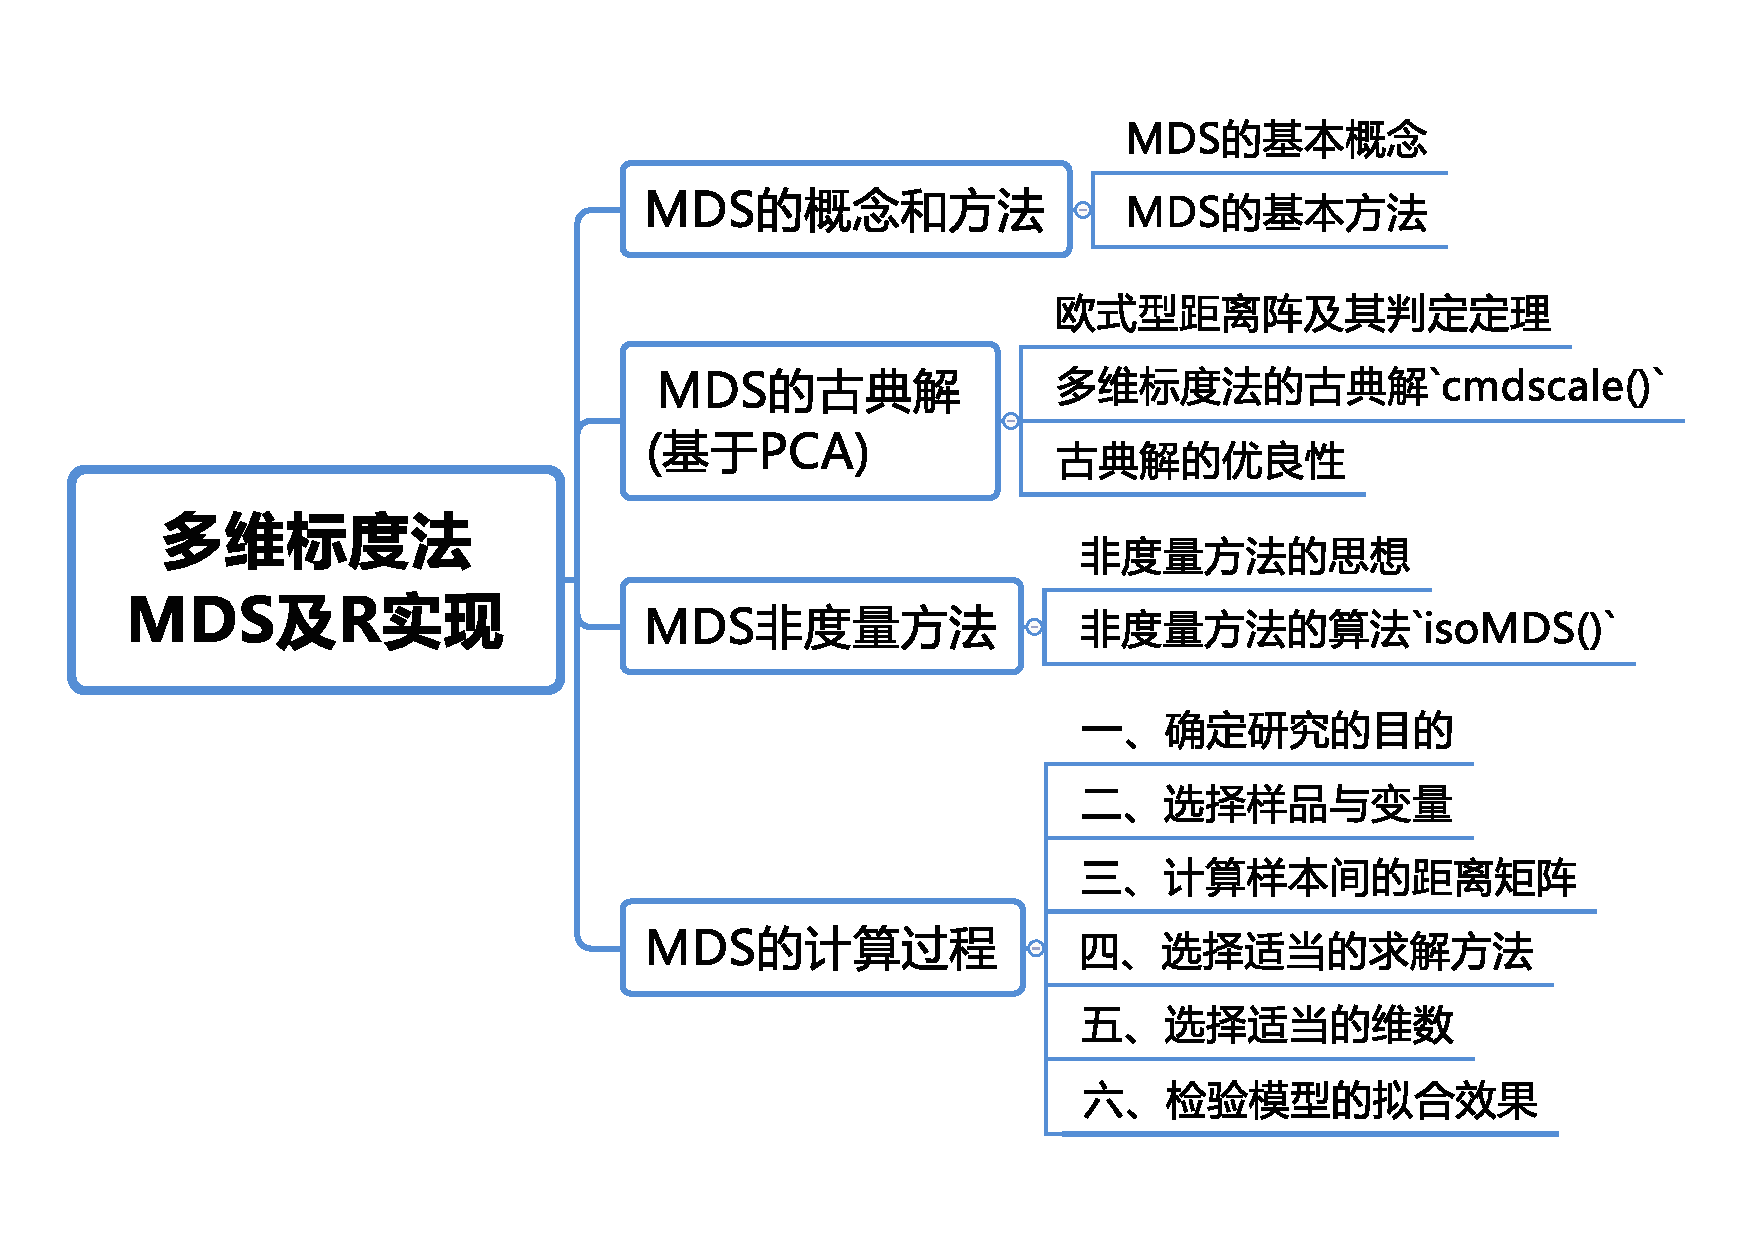
\includegraphics[width=12cm]{figures/xmind}
			\label{fig:xmind}
		\end{figure}

	\end{frame}
	
\section{\heiti 参考文献}

	\begin{frame}
	\frametitle{\heiti 参考文献}
	
		\begin{thebibliography}{Torgerson, 1958}
			\bibitem[王斌会, 2016]{王斌会2016}
			王斌会.
			\newblock {\em 多元统计分析及R语言建模(第四版)}.
			\newblock 暨南大学出版社, 2016.
			
			\bibitem[Torgerson, 1958]{Torgerson1958}
			Warren S.~Torgerson.
			\newblock Theory and Methods of Scaling.
			\newblock {\em New York: John Wiley}, 1958.
			
			\bibitem[Torgerson, 1958]{程其襄2010}
			程其襄, 张奠宙.
			\newblock {\em 实变函数与泛函分析基础(第三版)}.
			\newblock 高等教育出版社, 2010, pages 299--301.
		\end{thebibliography}
	\end{frame}
	
	\begin{frame}{\sffamily The End\qquad\qquad\qquad\qquad\qquad\qquad\qquad\qquad\qquad\ding{44}}
		\begin{center}
			\begin{tikzpicture}
			\node[above,xscale=1.2,yscale=1.4]{\Huge\bfseries 欢迎老师同学们批评指正!};
			\node[xscale=1.2,above,yscale=-1.4,scope fading=south,opacity=0.2]{\Huge\bfseries 欢迎老师同学们批评指正!};
			\end{tikzpicture}
		\end{center}
	\end{frame}
	
\end{document}